\documentclass[10pt,a4paper]{article}
\usepackage[utf8]{inputenc}
\usepackage[margin=1in]{geometry}
\thispagestyle{empty}

\usepackage[spanish]{babel}

\usepackage{amsmath}
\usepackage{amsfonts}
\usepackage{amssymb}

\usepackage{parskip}

\usepackage{listings}
\usepackage{xcolor}

\usepackage{enumerate}

\usepackage{hyperref}

\usepackage{float}
\usepackage{wrapfig}

\usepackage{graphicx}
\restylefloat{figure}

\usepackage[font=small,labelfont=bf]{caption}
\usepackage{subcaption}

\usepackage{cancel}

\usepackage{multicol}
\setlength{\columnsep}{22pt}

\usepackage{colortbl}
\usepackage{verbatim}

\DeclareMathOperator*{\argmin}{arg\,\min}
\DeclareMathOperator*{\argmax}{arg\,\max}

\usepackage{adjustbox}

\author{Cristian Escudero\\\small{Basado en el resumen de Guido Ghisolfi}}
\title{{\small Resumen Final}\\Auditoría en Informática}
\begin{document}

\definecolor{light-gray}{gray}{0.98}

\newcommand{\micaja}[1]{
\begin{center}
\marginbox{1pt}{
 \fcolorbox{lightgray}{light-gray}{
  \marginbox{1pt 3pt}{
   \begin{minipage}{0.93\textwidth}
   #1
   \end{minipage}%
  }
 }
}
\end{center}
}

\maketitle

\section{Control Interno y Auditoría Informática}

\subsection{Control Interno}

Las \texttt{EMPRESAS-ACTIVIDADES-ORGANISMOS} a lo largo del tiempo van sufriendo \textbf{cambios}, a partir de la infuencia de \textbf{tendencias externas}: \textit{globalización, avances tecnológicos, RR.HH., ideas, desafíos, ampliaciones/eliminaciones de ramas de negocio, fusiones con otras empresas}.

Ante la rapidez de los cambios, se requiere un buen \texttt{CONTROL} de todas las áreas y facetas de una empresa: \textit{producción, procesos, flujo de información}, y \textit{recursos} (humanos, materiales, etc).

\micaja{
Se puede definir \textbf{control interno} como: «cualquier actividad o acción realizada manual y/o automáticamente para prevenir, corregir errores o irregularides que puedan afectar al funcionanmiento de un sistema para conseguir sus objetivos.»
}

El \textbf{control} (actividad \textbf{continua }y \textbf{repetitiva}) se puede dar siempre que se sepa lo que se quiere, en base a:
\begin{multicols}{2}\begin{itemize}
\item Normas.
\item Procedimientos.
\item Estándares.
\item Objetivos deseados.
\end{itemize}
\end{multicols}

Su forma de incorporarlo subyace en dos opciones: 
\begin{multicols}{2}
\begin{itemize}
\item En cada actividad en particular.
\item Centralizado en un sector o área.
\end{itemize}
\end{multicols}

Los \textbf{tipos de control} que existen son:
\begin{itemize}
\item {\textbf{Controles preventivos.}} Para tratar de evitar el hecho (\textit{ejemplo: software de seguridad que impide entradas no-autorizadas}).
\item {\textbf{Controles detectivos.}} Cuando fallan los preventivos, para tratar de conocer cuanto antes el evento (\textit{ejemplo: registro de intentos de acceso no-autorizados}).
\item {\textbf{Controles correctivos.}} Facilitan la vuelta a la normalidad cuando se han producido incidencias (\textit{ejemplo: recuperación de un archivo dañado a partir de una copia de seguridad}).
\end{itemize}

Los límites del \textbf{control} los brindará el \texttt{costo/beneficio} de la empresa en cuestión, ya que es una actividad diaria para la misma. Es responsabilidad de la Dirección plantear una estrategia de inversiones en recursos informáticos así como implantar sistemas de controles internos de manera que se garanticen unos grados de eficiencia y seguridad sufcientes de los activos informáticos.

\subsection{Auditoría}

\micaja{
«Es la \textbf{actividad} consistente en la \textbf{emisión de una opinión profesional} sobre si el \textbf{objeto sometido a análisis} presenta \textbf{adecuadamente la realidad} que pretende \textbf{reflejar y/o cumple las condiciones} que le han sido prescriptas.»
}

Sólo tiene \textbf{validez} si la produce un profesional.  Es llevada a cabo cuando existe una \textbf{alta incertidumbre} de como están siendo llevadas las cosas (surge ante las \texttt{necesidades}, \texttt{problemas} o \texttt{dudas} que se presenten), y se realiza a pedido (por alguien que necesite la opinión). Es una tarea \textit{esporádica} o \textit{frecuente}, cuyo \textbf{alcance} es el objeto a analizar.

\micaja{
{ \small Una \textbf{auditoría} ataca a cualquier empresa, requiriendo saber en primera instancia cuáles son los \textit{controles}.}
}

\subsubsection{Tipos de auditoría}

\vspace{-1em}

\renewcommand{\arraystretch}{1.5}
\begin{table}[h]
    \begin{tabular}{lp{0.39\textwidth}p{0.39\textwidth}}
    \textbf{Tipo}         & \textbf{Objeto}                                              & \textbf{Finalidad}                                                \\
    \hline
    \textit{Financieras}  & Registros contables.                                & Adecúan a la realidad.                                   \\
    \hline
    \textit{Gestión}      & Toma de decisiones.                                 & Eficaz, eficiente, económico.             \\
    \hline
    \textit{Cumplimiento} & Normas, disposiciones, procedimientos, legislación (NDPL). & Adecúan a las NDPL.                 \\
    \hline
    \textit{Informática}  & \textit{Information Technology} (I.T.)                       & Eficiente y que se cumpla con NDPL. \\
    \hline
    \end{tabular}
\end{table}

Cada \textbf{tipo de auditoría} posee sus \texttt{procedimientos} para alcanzar el fin previsto.

\subsection{Control Interno Informático (C.I.I.)}

Controla \textbf{diariamente} que todas las actividades de I.T. son realizadas \textbf{cumpliendo los normas, estándares} y  \textbf{procedimientos} (NEP), fijados por la \textbf{Dirección de la Organización} y/o la \textbf{Dirección de Informática}, así como los requerimientos legales.

El C.I.I. está dotado de las personas y medios materiales proporcionados a los cometidos que se le encomienden.

\subsection{Auditoría informática (A.I.)}

\micaja{
«Proceso de \textbf{recolectar, agrupar y evaluar \texttt{evidencias}} para determinar si un \texttt{sistema informático} salvaguarda los \textbf{activos}, mantiene la \textbf{integridad de los datos}, lleva a cabo \textbf{eficazmente} los fines de la organización y utiliza \textbf{eficientemente} los recursos.»
}

\textbf{Sistema informático}: toda la tecnología del negocio. Todo lo que se maneja a través de la tecnología, no solamente el software.

\subsubsection{C.I.I. y A.I.: campos análogos}

\underline{\textbf{Similitudes:}}

\begin{itemize}
\item Personal con conocimientos específicos en I.T.
\item Verificación del cumplimiento de controles internos y NEP impuestos por la \textbf{conducción}.
\end{itemize}

\underline{\textbf{Diferencias:}}

\setlength{\tabcolsep}{13pt}
\begin{tabular}{p{.45\textwidth} p{.45\textwidth}}
 \underline{\textbf{\textit{Control Interno Informático}}}
& \underline{\textbf{\textit{Auditoría Informática}}}
\\
$\circ$ Análisis de los controles en el día a día.
&$\circ$ Análisis de un \textbf{momento} informático determinado.
\\ 
$\circ$ Informa a la Dirección del Departamento de Informática.
&$\circ$ Informa a la Dirección General.
\\
$\circ$ Solo personal interno.
&$\circ$ Personal interno y externo.
\\
$\circ$ El alcance de sus funciones es únicamente sobre el Departamento de Informática.
&$\circ$ Tiene cobertura sobre todos los componentes de los \textit{sistemas de información} de la organización.
\end{tabular}

\subsubsection{Metodología de la A.I.}

Conjunto de métodos para llevar adelante una A.I.:

\begin{enumerate}
\item \textbf{Definición del objeto de la auditoría.} 
\item \textbf{Toma de contacto.} Conocer la organización, organigrama funcional, y conocer en detalle el sector de tecnología (\textit{funciones, sectores, recursos humanos, tecnológicos y económicos}).
\item \textbf{Procedimientos y normas.} Desde el \textit{acto de apertura de auditoría} al \textit{acto de cierre}.
\item \textbf{Tipos de A.I.} Puede ser \textit{completa}, sobre un determinado sistema, o una mezcla. Puede realizarse una comprobación de las acciones correctivas de auditorías anteriores.
\item \textbf{Realizar la/s auditoría/s.}
\item \textbf{Presentación de las conclusiones.} De forma simultánea o secuencial. De manera formal y/o visual (muestra los hallazgos de su trabajo a una audiencia).
\item \textbf{Soluciones alternativas a los problemas.} Es decir, proponer hacer algo en un cierto tiempo estimado bajo un determinado costo. Lo más importante es que sean soluciones adecuadas a la \textbf{realidad} de la empresa.
\end{enumerate}

\underline{Nota:} al hacer una A.I., hay que tratar de mantener objetividad y disciplina. Toda la actividad del auditor quedará reflejada en los \texttt{PAPELES DE TRABAJO}.


\subsubsection{El Informe de Auditoría}

Aspectos a tener en cuenta:

\begin{itemize}
\item \textbf{Normas.}
\item \textbf{Evidencias.} La opinión debe estar basada en evidencias justificativas.
\item \textbf{Irregularidades.} O sea, fraudes y errores. Es necesario diseñar pruebas antifraude.
\item \textbf{Documentación.} El informe debe estar basado en los \textbf{papeles de trabajo}, o sea, a la totalidad de documentos preparados o recibidos por el auditor, que en conjunto constituyen un compedio de la información utilizada y de las pruebas efectuadas, juntos a las decisiones tomadas para llegar a formarse la opinión. Constituyen el conocimiento del auditor y pueden llegar a tener valor en el tribunal de justicia. 

Se incluye dentro de estos documentos: \textit{el contrato entre el cliente y el auditor, las declaraciones de la dirección vinculadas con los objetivos a auditar, informes de terceras personas vinculadas al mismo}.
\item \textbf{Informe.} Es la comunicación formal al cliente de: \textit{alcances, resultados} y \textit{conclusiones}.
\end{itemize}

\subsubsection*{\underline{\textbf{Contenidos del informe:}}}

\begin{enumerate}
\item \textbf{Identificación del informe.} Título para distinguirlo de otros informes.
\item \textbf{Identificación del cliente.} Destinatario que solicita el trabajo.
\item \textbf{Identificación de la empresa a auditar.} Entidad objeto de la auditoría.
\item \textbf{Objetivos de la auditoría.} Para identificar su propósito, señalando los objetivos incumplidos.
\item \textbf{Normativas aplicadas y excepciones.} Todo lo que se tuvo en cuenta al realizar la A.I.
\item \textbf{Alcance auditoría.} Área organizativa, período de auditoría y limitación al alcance y restricciones del auditado.
\item \textbf{Conclusiones.} Informe corto de opinión, conteniendo los \textbf{puntos favorables} y \textbf{desfavorables}.
\item \textbf{Resultados.} Informe extenso, incluye plan de acción.
\item \textbf{Informes previos.} No es practica recomendable.
\item \textbf{Fecha del informe.} Inicio y fin del trabajo.
\item \textbf{Identificación y firma del auditor.}
\item \textbf{Distribución del informe.} Quienes podrán hacer uso del mismo.
\end{enumerate}
 
\section{Organización del Departamento de Auditoría Informática}

\subsection{Historia de la tecnología en las empresas}

\begin{wrapfigure}{r}{0.5\textwidth}
  \caption{El Departamento Tecnológico es el que posee más recursos 
						económicos y es denominado el “Corazón de la 							empresa”. También denominado: Departamento 
						tecnológico, Centro de cómputos o Dep de inf.}
  \label{fig:st}
  \centerline{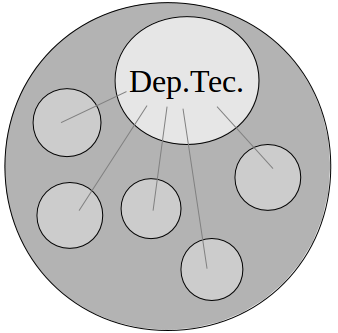
\includegraphics[width=0.3\textwidth-\fboxrule-\fboxrule]{img/st.png}}
\end{wrapfigure}

Hace sesenta años no existía la tecnología, el trabajo era manual y se almacenaba la información en papeles y registros. Con el surgimiento de la computación, el auditor tenía la necesidad de estudiar informática o contratar a un ayudante para que le brinde información.
En la actualidad las empresas destinan importantes recursos en el sector tecnológico, volviéndose altamente dependientes del mismo, de tal forma que este domina su funcionamiento.

La tendencia futura de la auditoría informática radicará en los siguientes principios: todos los auditores deberán tener conocimientos informáticos; a la vez de mayor necesidad de especialistas con conocimiento cada vez más específico; y por último a la necesidad de un título profesional de auditor informático.

Para el buen funcionamiento del sector es necesario el \textbf{control interno}. Cuando surgen más problemas, lo recomendable es realizar una auditoría informática. En la actualidad, el auditor es experto en tecnologías y lo que antes era un auditor con un ayudante en tecnologías, ahora es un experto en tecnologías con ayudantes en las demás áreas: económicas, financieras, etc.

\subsection{Perfil del Auditor Informático}

Se deberán contemplar las siguientes características para mantener un profesional adecuado y actualizado:
\begin{enumerate}
\item Conocimiento básicos en:
\begin{multicols}{2}
\begin{itemize}
\item Desarrollo informático, gestión de proyectos y ciclos de vida de proyectos de desarrollo tecnológico.
\item Gestión del departamento de tecnología.
\item Análisis de riesgos en un entorno informático.
\item Sistemas operativos.
\item Telecomunicaciones.
\item Gestión de base de datos.
\item Redes locales.
\item Seguridad física.
\item Gestión de la seguridad y continuidad del negocio.
\item Gestión de problemas y cambios.
\item Administración de datos.
\item Ofimática.
\item Comercio electrónico.
\item Encriptación de datos.
\end{itemize}
\end{multicols}
\item Técnicas de gestión empresarial y conocimientos financieros del negocio.
\item Conocimiento del concepto de Calidad Total.
\end{enumerate}

\subsection{Funciones a desarrollar por la Auditoría Informática}

La función Auditoría Informática debe mantener en la medida de lo posible los objetivos de revisión que le demande la organización, abarcando campos de revisión como el C.I.I. de los servicios y de las aplicaciones.

\micaja{
El \textbf{auditor informático} es responsable para establecer los OdC que reduzcan o eliminen la exposición al riesgo de control interno. El auditor deberá revisar los controles y evaluar resultados de su revisión para determinar correcciones y mejoras. Tiene además la obligación de proveer procedimientos y observaciones para mejorar la efectividad, eficacia y medición del riesgo empresarial.
}

\section{Auditoría de la Dirección}

Algunas actividades básicas de todo proceso de dirección son: \textit{planificar, organizar, coordinar y controlar.}

\subsection{¿Cómo se debería trabajar en un Centro de Computo?}

\begin{enumerate}
\item {\textbf{Planificar}} la conducción del área. Se trata de preveer la utilización de las I.T. en la empresa.
\begin{itemize}
\item \textbf{Plan Estratégico de Tecnología} ó PEdT (proyectar a no más de tres años, ya que la tecnología cambia muy rápido). Tener en cuenta la situación actual, la cultura organizacional, el sector de la actividad y las acciones de la competencia. Debe asegurar el alineamiento de los \textit{sistemas de información} con los objetivos en la empresa.
\item \textbf{Plan Operativo Anual.} Uno por cada año que se tenga planificado el PEdT. Se establece al comienzo de cada ejercicio y marca las pautas a seguir durante el mismo.
\item \textbf{Plan de Contingencia.} Contra algo que no esperamos que suceda y pueda ser de gran impacto, haciendo que peligre el funcionamiento de la empresa (\textit{ejemplos: inundación, incendio, atentados, robos, ataques}). Ha de contener todo lo necesario para que permita la \textbf{continuidad} del negocio.
\end{itemize}
\item {\textbf{Organizar y coordinar.}} Sirve para estructurar los recursos, los flujos de información y los controles que permitan alcanzar los \textbf{objetivos} de la empresa.
\begin{enumerate}[2.1.]
\item \textbf{Comité de informática.} En él debe haber representantes de todas las áreas usuarias y departamentos. Un auditor va a preguntar si existe un comité (si no, pedirá la creación de uno) y ver las decisiones tomadas por el mismo.
Las funciones del comité son:
\begin{itemize}
\item Aprobación del PEdT.
\item Aprobación de grandes inversiones en tecnología.
\item Fijación de prioridades entre los grandes proyectos informáticos.
\item Vehículo de discusión entre informáticos y sus usuarios.
\item Vigilancia y seguimiento de la actividad del Departamento de Informática.
\end{itemize}
\item \textbf{Ubicación del Departamento de Informática en la empresa.} El auditor revisará su emplazamiento organizativo y su independencia de los otros departamentos.
\item \textbf{Descripción de funciones y responsabilidades del Departamento de Informática.} Funciones descritas y responsabilidades claramente delimitadas y documentadas. Ambas deben estar extendidas a todo el personal de informática. Además, ha de haber una \textbf{división entre funciones y responsabilidades}: se debe impedir que un solo individuo pueda transformar un proceso crítico. Entre las funciones, se listan:
\begin{multicols}{3}
\begin{itemize}
\item Administración de BD.
\item A.I.
\item C.I.I.
\item Capacitación.
\item Desarrollo.
\item Mantenimiento.
\item Redes.
\item Seguridad.
\end{itemize}
\end{multicols}
\item \textbf{Estándares de funcionamiento y procedimientos.} Formentar, documentar y difundir. El auditor evaluará su existencia y adecuamiento (\textit{por ejemplo, mediante entrevistas}).
\item \textbf{Gestión de recursos humanos.} El auditor revisará que sea llevado correctamente. Una forma es mantener estándares para:
\begin{multicols}{2}
\begin{itemize}
\item Proceso de selección: formalmente escrito.
\item Evaluación de desempeño.
\item Formación.
\item Motivación.
\item Promoción.
\item Finalización de contrato.
\end{itemize}
\end{multicols}
\item \textbf{Comunicación}. Efectiva y eficiente entre Dirección de Tecnología y el personal.
\item \textbf{Gestión económica.}
\begin{itemize}
\item \textit{Presupuestos económico:} que exista y sea adecuado, en línea con los planes estratégicos y operativos del Departamento.
\item \textit{Adquisición de bienes y servicios.}
\item \textit{Medida y reparto de costos:} evaluar su existencia y que este sea correcto.
\end{itemize}
\item \textbf{Seguros.} Tener cobertura para sistemas críticos o medir alternativas. Normalmente se aplica a empresas grandes.
\end{enumerate}
\item \textbf{Controlar.} Efectuar un seguimiento \textbf{permanente} de las distintas actividades del Departamento de Tecnología, y que esté asegurado el \textbf{cumplimiento de la normativa legal} (ejemplos: \textit{protección de datos personales, contratos de comercio electrónico, normativa emitida por órganos reguladores}).
\end{enumerate}

\section{Auditoría de la Seguridad Física}

\micaja{
La \texttt{SEGURIDAD FÍSICA} \textbf{garantiza} la \textbf{integridad} de los activos humanos, lógicos y materiales de un \textbf{Centro de Cómputos}. Se deben tener medidas para atender los \textbf{riesgos de fallos}, local o general, según la \textbf{cronología del fallo} (antes, durante y después).
}

La \textbf{auditoría} es el medio que va a proporcionar la evidencia o no de la Seguridad Física en el ámbito en el que se va a desarrollar la labor profesional. La Auditoría Física no difiere de la auditoría general más que en el \textbf{alcance} de la misma.

\subsection{Antes del fallo}

Obtener y \textbf{mantener un nivel adecuado} de seguridad física sobre los activos. Ha tener en cuenta:
\begin{multicols}{2}
\begin{itemize}
\item Ubicación del edificio.
\item Ubicación del Centro de Cómputos dentro del edificio.
\item Compartimentación.
\item Elementos de construcción. Perímetro físico.
\item Potencia eléctrica. Generación de energía.
\item Sistemas contra incendios.
\item Control de acceso (ingreso/egreso).
\item Selección del personal.
\item Seguridad de los medios.
\item Medidas de protección.
\item Duplicación de medios.
\end{itemize}
\end{multicols}

\subsection{Durante el fallo}

Ejecutar un \texttt{PLAN DE CONTINGENCIA} adecuado. El mismo está formado por un \textbf{plan de recuperación ante desastres} más \textbf{un centro alternativo de cómputos}.

El plan de recuperación ante desastres debe:
\begin{itemize}
\item \textbf{Realizar un análisis de riesgos}  \textbf{de sistemas críticos} (computadora, software, RR.HH.).
\item Establecer un \textbf{período crítico} de recuperación.
\item Realizar un análisis de aplicaciones críticas, \textbf{priorizando procesos}.
\item Determinar las prioridades de procesos \textbf{por día} y su \textbf{orden}.
\item Establecer objetivos de recuperación (\textit{tiempo de interrupción}).
\item Asegurar capacidad de comunicaciones y servicios de backups.
\end{itemize}

\subsection{Después del fallo}

Los contratos de seguros pueden compensar en mayor o menor medida las perdidas, gastos o responsabilidades que se puedan derivar una vez detectado y corregido el fallo.

Gama de seguros a contemplar:
\begin{itemize}
\item Cobertura por daño físico en los equipos.
\item Reconstrucción de medios de software.
\item Gastos extras (ejecución del plan de contingencia).
\item Pérdida, robo, o daño de documentos y registros valiosos.
\item Errores u omisiones de profesionales que ocasionen pérdidas.
\item Cobertura de fidelidad con actos deshonestos o fraudulentos de los empleados.
\item Transporte de medios ante perdida o daño en el transporte.
\item Contratos con proveedores y de mantenimiento que aseguran \textbf{repuestos}.
\end{itemize}

\subsection{Áreas de la Seguridad Física}

Las áreas en las que el auditor ha de interesarse son:
\begin{itemize}
\item \textbf{Centro de proceso de datos e instalaciones.} Entorno, sala de Host, sala de Operadores, sala de Impresoras, cámara acorazada, oficinas, almacenes, instalaciones eléctricas, aire acondicionado, área de descaso y servicio.
\item \textbf{Equipos y comunicaciones.} Host, terminales, computadoras personales, equipos de almacenamiento masivo de datos, impresoras, medios y sistemas de telecomunicaciones. Se ha de inspeccionar su \textbf{ubicación} y \textbf{acceso}.
\item \textbf{Seguridad física del personal.} Accesos y salidas seguras, medios y rutas de evacuación, extinción de incendios, sistemas de bloqueo de puertas y ventanas. Normas y políticas emitidas y distribuídas al personal referente al \textbf{uso de instalaciones} por parte de éste.
\end{itemize}

\subsection{Fuentes de la Auditoría Física}

Para evaluar la Seguridad Física, las siguientes fuentes han de estar accesibles en todo CPD:

\begin{itemize}
\item Política, normas y planes de seguridad.
\item Auditorías anteriores, generales y parciales.
\item Contratos de seguros, de proveedores y de mantenimiento.
\item Actas e informes de técnicos y consultores (edificio, electricidad, aire/calefacción).
\item Informe de accesos y visitas.
\item Informes sobre pruebas de evacuación.
\item Políticas del personal.
\item Inventario de soportes (backups, control de copias, etc).
\item Inventario de tecnologías en general.
\end{itemize}

\subsection{Herramientas y Técnicas del Auditor:}

\begin{multicols}{2}
\begin{enumerate}
\item Observación
\item Lectura de documentación.
\item Entrevistas.
\item Consultas o asesoramientos.
\item Cámaras de video/fotográfica.
\item Cuaderno de campo/grabadora de audio.
\end{enumerate}
\end{multicols}

\subsection{Riesgos}

\begin{itemize}
\item Ingresos no autorizados.
\item Daños en los equipos.
\item Atentados sobre equipos, instalaciones, documentación.
\item Robos de equipos, documentos, sistemas, programas.
\item Copiado y/o divulgación de información sensible.
\end{itemize}

\subsection{Recomendaciones}

\begin{itemize}
\item Instalaciones \textbf{claves}: ubicarse en lugares a los cuales no puede acceder el público.
\item Edificios discretos y con señalamiento mínimos de su propósito.
\item Equipamiento de soporte (fax, fotocopiadoras) deben ubicarse adecuadamente y controlar su acceso.
\item Implementación de un sistema de detección de intrusos según estándares reconocidos.
\item Materiales peligrosos o combustibles deben \textbf{almacenarse} en lugares seguros.
\item Seguridad ambiental: analizar normativas referidas a comer, beber y fumar en áreas tecnológicas.
\item Mantener \textbf{registro} de  todas las \textbf{fallas} y de toda \textbf{actividad} vinculada con el mantenimiento preventivo y correctivo.
\item Implementar controles cuando se retiran equipos de la sede de la organización para sus diversos fines.
\item Considerar impacto de eventuales desastres en zonas próximas.
\item Políticas de escritorio limpio: no dejar material que pueda ser confidencial (que pueda ser sustraído, robado, o fotocopiado).
\item Política de pantallas limpias (dejar las mismas bloqueadas).
\item Guardar bajo llave documentos y medios informáticos.
\item \textbf{No} dejar conectadas PCs, terminales e impresoras al estar desatendidas.
\item Proteger puntos de recepción y envío de fax/correo.
\end{itemize}


\section{Auditoría del Desarrollo de Aplicaciones}

\micaja{
La \texttt{INGENIERÍA DE SOFTWARE} (IS) puede ser entendida como el establecimiento y uso de \textbf{principios} de \textbf{ingeniería robustos}, orientados a obtener SW económico que sea fiable, cumpla los requisitos previamente establecidos y funcione de manera eficiente sobre la arquitectura esperada.
}

\micaja{
El \texttt{DESARROLLO} incluye \textbf{todo el ciclo de vida} del SW, excepto explotación, mantenimiento y la desafección o eliminación del mismo.
}

Para \textbf{auditar el desarrollo de aplicaciones} hay que verificar la existencia de controles internos que garanticen la construcción de SW basado en los \textbf{principios de IS}.

\subsection{Importancia de la Auditoría del Desarrollo}

\begin{itemize}
\item Los avances tecnológicos han hecho que el desafío mas importante y el principal factor de éxito de la informática sea la mejora de la \textbf{calidad del SW}.
\item Gasto destinado a SW es cada vez mayor al dedicado al HW.
\item El SW como producto es muy difícil de validar. A mayor control, mayor calidad y menor coste de mantenimiento.
\item Hace unos años, se produjo la denominada ``\textbf{crisis del SW}'' (1970-1990). Estadísticas internacionales:
\begin{itemize}
\item \textbf{1.5\%}: Se usó tal y como se entregó.
\item \textbf{3.0\%}: Se usó después de algunos cambios.
\item \textbf{19.5\%}: Se usó y luego se abandonó o se rehizo.
\item \textbf{47.0\%}: Se entregó pero nunca se usó.
\item \textbf{29.0\%}: Se pagó pero nunca se entregó.
\end{itemize}
\item Aplicaciones informáticas pasan a ser un activo muy importante para la gestión.
\end{itemize}

\subsection{Planteamiento y metodología}

Las funciones que tradicionalmente se asignan al área de desarrollo son:
\begin{itemize}
\item Planificación del área y participación en la elaboración del PEdT.
\item Desarrollo de nuevos sistemas.
\item Estudios de \textbf{nuevos lenguajes}, técnicas, metodologías, estándares, herramientas relacionadas con el desarrollo y adopción de los mismos cuando sea oportuno para mantener un nivel de vigencia adecuado a la tecnología del momento.
\item Establecer un plan de formación para el personal del área.
\item Establecer normas y controles para las actividades del área y comprobar su observancia.
\end{itemize}

Se puede desglosar la auditoría del desarrollo en dos grandes apartados:
\begin{enumerate}
\item \textbf{Auditoría de la organización y gestión del área de desarrollo.}
\item \textbf{Auditoría de proyectos de desarrollo de sistemas de información.}
\end{enumerate}

Partiendo de los riesgos potenciales que existen, se determinan una serie de \textbf{objetivos de control} (OdC) que los minimicen. Para cada OdC se han de especificar los controles que contribuyan a lograr su cumplimiento, junto a una serie de pruebas que comprueben la existencia y correcta aplicación de estos controles.

Una vez fijados los OdC, será función del auditor determinar el grado de cumplimiento de cada uno de ellos, y de los controles asociados.

\subsection{Auditoría de la Organización y Gestión del Área de Desarrollo}

Se consideran los siguientes objetivos de control:
\begin{multicols}{2}
\begin{enumerate}
\item El área de desarrollo debe tener \textbf{objetivos asignados} dentro del departamento y \textbf{una organización} que le permita el cumplimiento de los mismos.
\item El personal del área de desarrollo debe contar con la \textbf{formación} adecuada y estar \textbf{motivado} para la realización del trabajo.
\item Si existe un \textbf{plan de sistemas}, los proyectos que se lleven a cabo se basarán en dicho plan y lo mantendrán actualizado.
\item La propuesta y aprobación de nuevos proyectos debe realizarse de forma reglada.
\item La asignación de \textbf{recursos a los proyectos} debe hacerse de forma reglada.
\item El \textbf{desarrollo de sistemas de información} debe hacerse aplicando principios de la IS ampliamente aceptados.
\item Las \textbf{relaciones con el exterior} del departamento tienen que producirse de acuerdo a un procedimiento.
\item La \textbf{organización} del área debe estar \textbf{siempre adaptada} a las necesidades de cada momento.
\end{enumerate}
\end{multicols}

\subsection{Auditoría de Proyectos de Desarrollo de Sistemas de Información}

La auditoría de un proyecto de desarrollo se puede hacer a medida que avanza el proyecto, o una vez finalizado el mismo. La diferencia es que en el primer caso el auditor puede afectar el desarrollo del mismo mediante sugerencias y observaciones.

Se consideran las siguientes fases dentro del desarrollo de S.I., en las cuales el auditor planteará los correspondientes OdC:
\begin{multicols}{2}
\begin{enumerate}
\item \textbf{Aprobación, planificación y gestión del proyecto.}
\item \textbf{Análisis.}
\item \textbf{Diseño.}
\item \textbf{Construcción.}
\item \textbf{Implantación.}
\end{enumerate}
\end{multicols}


\begin{comment}
Cuestiones de repaso:

Capitulo1:
1. Cuales son los elementos fundamentales del concepto de auditoría?
2. Cuantas clases diferentes de auditoría existen?
3. Que sector es uno de los principales usuarios de la auditoría?
4. Que ventajas aporta el computador respecto al trabajo manual?
5. Que significan las siglas CAAT?
6. En que afecta a los auditores la introducción de las TI en los sistemas de información?
7. Que diferencias hay entre auditoría y consultoría?
8. Cuales son las ventajas de la informática como herramienta de auditoría financiera?
9. Que pueden aportar los sistemas expertos a la auditoría informática?
10. Cuáles son las razones de la baja utilización de las TI como herramienta de la auditoría financiera?
Capitulo 2:
1. Que cambios en la empresa provocan tensión en el control interno existente?
2. Cuales son las funciones del control interno informático?
3. Cuales son los objetivos de la auditoría informática?
4. Cuales son las semejanzas y diferencias entre el control interno y la auditoría informática?
5. Ponga ejemplos de controles correctivos en diversas áreas informáticas.
6. Cuales son los principales controles en el área de desarrollo?
7. Que procesos definiría para controlar la informática distribuida y las redes?
8. Que controles se deberían establecer en las aplicaciones?
9. Como justificaría ante un directivo de la empresa la inversión necesaria en control y auditoría informática?
10. Describa la información como modo de la estructuración de las empresas.  
Capitulo 3:
1. Que diferencias y similitudes existen entre las metodologías cualitativas y cuantitativas? Que ventajas y que inconvenientes tienen?
2. Cuales son los componentes de una contra medida o control (pirámide de la seguridad)? Que papel desempeñan las herramientas de control? Cuales son las herramientas de control mas frecuentes?
3. Que tipos de metodologías de plan de contingencias existen?  En que se diferencian? Que es un plan de contingencias?
4. Que metodologías de auditoría informática existen? Para que se usa cada una?
5. Que es el nivel de exposición y para que sirve?
6. Que diferencias existen entre las figuras de auditoría informática y control interno informático? Cuales son las funciones mas importantes de este?
7. Cuales son las dos metodologías mas importantes para el control interno informático? Para que sirve cada una?
8. Que papel tienen las herramientas de control en los controles?
9. Cuales son los objetivos de control en el acceso lógico?
10. Que es el single sign on? Por que es necesario un SW especial para el control de acceso en los entornos distribuidos?
Capitulo 4:
1. Que diferencias existen entre evidencia suficiente y adecuada?
2. Que diferencias existen entre prueba de cumplimiento y prueba sustantivo?
3. Que diferencias existen entre opinión desfavorable y denegada?
4. Que significa importancia relativa? Y materialidad?
5. Que significado tiene la responsabilidad civil del auditor informático emisor del informe de auditoría informática y el firmante del mismo?
6. Cual es la utilidad del documento denominado declaraciones de dirección?
7. Que diferencia existe entre experto informática y auditor informático?
8. Que diferencia existe entre auditor interno y externo?
Capitulo 5:
1. Cuales son las lineas de evolución de la auditoría informática?
2. Que diferentes acepciones existen en la auditoría informática?
3. Cual es el perfil del auditor informático general?
4. Que formación debe poseer el auditor informático?
5. Cuales son las funciones de la auditoría informática?
6. Que aspectos pueden hacer mas compleja, en la actualidad, la función de auditoría informática?
7. Cual debe ser la localización de la función de auditoría informática en la empresa?
8. Cuales son las tareas del jefe del departamento de auditoría informática?
9. Que tamaño debe tener el departamento de auditoría informática?
10. Defina un plan de formación para que un informático pueda desempeñar sin problemas la función del auditor. 
Capitulo 8:   
1. Diferencie entre seguridad lógica, física y de las comunicaciones, poniendo varios ejemplos de cada tipo.
2. Explique el concepto de nivel adecuado de seguridad física.
3. Como definiría los que constituye un desastre?
4. Que tipos de seguros existen?
5. Que medios de extinción de fuego conoce?
6. Por que es importante la existencia de un sistema de control de entradas y salidas?
7. Que técnicas cree que son las mas adecuadas para la auditoría física?
8. Cuales suelen ser las responsabilidades del auditor informático interno respecto a la auditoría física?
9. Que aspectos considera mas importantes a la hora de auditar el plan de contingencia desde el punto de vista de la auditoría física?
10. Que riesgos habría que controlar en el centro de proceso alternativo?
Capitulo 10:
1. Descríbanse las actividades a realizar por un auditor para evaluar un plan estratégico de sistemas de información.
2. Descríbanse las funciones de un comité de informática. Elabórese una lista con las funciones empresariales que deberían estar representadas en dicho comité. Que objetivo
3. Descríbanse las ventajas de tener procedimientos. Elabórese un guión de lo que podrían ser procedimientos de a) diseño de sistemas, b) programación.
4. Que evidencias deberá buscar el auditor para poder evaluar si las necesidades 


\end{comment}


\end{document}
